\RequirePackage{fix-cm}
\documentclass[english]{article}
\usepackage[LGR,T1]{fontenc}
\usepackage[latin9]{inputenc}
\setlength{\parskip}{\medskipamount}
\setlength{\parindent}{0pt}
\usepackage{amsmath}
\usepackage{amssymb}
\usepackage{fixltx2e}
\usepackage{graphicx}
\usepackage{subfigure}

%sequenz-diagramm
\usepackage{tikz}
\usetikzlibrary{arrows,shadows}

%code snippets
\usepackage{color}
\usepackage{listings}
\usepackage{courier}
\usepackage{caption}
\usepackage{pgf-umlsd}
 \lstset{
         basicstyle=\footnotesize\ttfamily, % Standardschrift
         %numbers=left,               % Ort der Zeilennummern
         numberstyle=\tiny,          % Stil der Zeilennummern
         %stepnumber=2,               % Abstand zwischen den Zeilennummern
         numbersep=5pt,              % Abstand der Nummern zum Text
         tabsize=2,                  % Groesse von Tabs
         extendedchars=true,         %
         breaklines=true,            % Zeilen werden Umgebrochen
         keywordstyle=\color{red},
            frame=b,         
 %        keywordstyle=[1]\textbf,    % Stil der Keywords
 %        keywordstyle=[2]\textbf,    %
 %        keywordstyle=[3]\textbf,    %
 %        keywordstyle=[4]\textbf,   \sqrt{\sqrt{}} %
         stringstyle=\color{white}\ttfamily, % Farbe der String
         showspaces=false,           % Leerzeichen anzeigen ?
         showtabs=false,             % Tabs anzeigen ?
         xleftmargin=17pt,
         framexleftmargin=17pt,
         framexrightmargin=5pt,
         framexbottommargin=4pt,
         %backgroundcolor=\color{lightgray},
         showstringspaces=false      % Leerzeichen in Strings anzeigen ?        
 }
 \lstloadlanguages{% Check Dokumentation for further languages ...
         %[Visual]Basic
         %Pascal
         %C
         C++
         %XML
         %HTML
         %Java
 }
    %\DeclareCaptionFont{blue}{\color{blue}} 

  %\captionsetup[lstlisting]{singlelinecheck=false, labelfont={blue}, textfont={blue}}
\DeclareCaptionFont{white}{\color{white}}
\DeclareCaptionFormat{listing}{\colorbox[cmyk]{0.43, 0.35, 0.35,0.01}{\parbox{\textwidth}{\hspace{15pt}#1#2#3}}}
\captionsetup[lstlisting]{format=listing,labelfont=white,textfont=white, singlelinecheck=false, margin=0pt, font={bf,footnotesize}}
% code snippets end ############################################

\makeatletter

%%%%%%%%%%%%%%%%%%%%%%%%%%%%%% LyX specific LaTeX commands.
\DeclareRobustCommand{\greektext}{%
  \fontencoding{LGR}\selectfont\def\encodingdefault{LGR}}
\DeclareRobustCommand{\textgreek}[1]{\leavevmode{\greektext #1}}
\DeclareFontEncoding{LGR}{}{}
\DeclareTextSymbol{\~}{LGR}{126}

%%%%%%%%%%%%%%%%%%%%%%%%%%%%%% Textclass specific LaTeX commands.
\numberwithin{equation}{section}
\numberwithin{figure}{section}
\numberwithin{table}{section}

\makeatother

\usepackage{babel}
\begin{document}

\title{Automated Routing in Pedestrian Dynamics
Fachhochschule Aachen, Campus J�lich
Medizintechnik und Technomathematik,
Technomathematik}


\author{Masterthesis from Arne Graf}


\date{2015-10-06}
\pagenumbering{gobble}% Remove page numbers (and reset to 1)
\maketitle
\newpage

\begin{titlepage}
\centering
\vspace{3cm}

{\huge 
Automated Routing in Pedestrian Dynamics
}

\vspace{3 cm}
Fachhochschule Aachen, Campus J�lich

Medizintechnik und Technomathematik,

Technomathematik

\vspace{3 cm}

Masterthesis from Arne Graf

2015-10-06

\end{titlepage}

\newpage
\pagenumbering{arabic}% Arabic page numbers (and reset to 1)
\section*{Abstract}
%In dieser Arbeit wird genommen: Model von Felix, Bodenfeld von Madrid, Code adaptiert von Leonardo Andr�s Zepeda N��ez. 
%Es wird ein Testmodel beschrieben, welches den Einflu� des Madrid-Bodenfeldes untersucht.
%Historie: Dietrich's Model in Jupedsim; Bodenfeld warf Frage auf: Welche Diskretisierung (rectGrid, triangulated, how to deal with wall-surfaces), Probleme durch non-smooth Bodenfeld (?); -> Beschluss: Bodenfeld so gestalten, dass es gute Eigenschaften bei der Fu�g�ngersimulation verspricht. 
%Dieses dann untersuchen und qualifizieren. Durch die Betreuung von M.C. floss die Erfahrung zahlreicher Modelle ein und es gelang bei der Modelfindung ein geeignetes Testmodel neu zu beschreiben.

In this thesis, the effect of an alternate floor-field was analyzed, by using it in a newly composed test-model for pedestrian dynamics. In the simulation of pedestrian (crowd) movement, the routing of agents\footnote{An agent is the representation of a pedestrian in the simulation. Depending on the used model, an agent incorporates some kind of artificial intelligence or basic agent-attributes only (like size, speed attributes, etc.). In the latter case the model takes over the task of navigating agents.} is an integral part. Routing can be seen as the composition of two aspects: the global pathfinding through a geometry and the avoidance of static or dynamic obstacles\footnote{collision detection} (like walls or other agents) in a local\footnote{local in time and/or in space} situation.

The history of pedestrian simulation shows various models with different answers to the question of navigation. Many of which make use of manually added elements\footnote{like some sort of domain-decomposition, e.g. through helplines} to solve the global pathfinding, which enable the user to simulate crowd movement in that very geometry. Other models use an automated algorithm, that will supply a navigation direction calculated from the agent's current position, the goal (area) and the geometry data. The model described by Dietrich is one of the later. It uses the solution of the Eikonal Equation (see chapter \ref{eikonalequation}), which describes a 2-D wave-propagation. The wave starts in the target region and propagates through the geometry. To navigate agents, they are directed in the opposite direction of the gradient of said solution of the Eikonal Equation. It is to be noted, that the solution of the Eikonal Equation can be calculated beforehand and does not contribute to the runtime of any given simulation scenario. The Routing using the plain floor-field will yield non-smooth pathways as described later. This could pose a problem for some models. Dietrich shows the existance and uniqueness of his problem-formulation by using the theorem of Picard-Lindel�f.
\footnote{Picard-Lindel�f theorem: Consider the initial value problem \newline \begin{center}
$y'(t) = f(t,y(t)), \quad y(t_0 ) = y_0, \quad t \in [t_0 - \epsilon, t_0 + \epsilon]$.\newline
\end{center}  Suppose $f$ is uniformly Lipschitz continuous in y and continuous in $t$. Then, for some value $\epsilon > 0$, there exists a unique solution $y(t)$ to the initial value problem on the interval $[t_0 - \epsilon, t_0 + \epsilon]$.}
To apply this theorem, Lipschitz-continuous first derivatives of the input-functions must be given. Dietrich solves that problem by the use of a mollifier, which basically takes a locally integrable function and returns a smooth approximation.

In this thesis, a different floor-field is described, which solves above issue (non-smoothness) as a welcome side-effect. The research-group in Madrid (add ref) is working on the safe navigation of robots. They are not to follow paths, which cut corners (which come close to any obstacles). A so-called distance-field is created and used as we see later. The welcome side-effect is in \emph{smooth} pathways through the avoidance of walls and corners. The researchers take that approach even further, by reducing any geometry into a graph of edges and knots and thus having the domain in which the 2-D wave propagates reduced dramatically. Their intent is to re-calculate the floor-field in real-time using it for the reduced view-field of the robot's sensors.
Our interest in this sleight of hand is different. We welcome the smoothness of the resulting pathways and take special interest in the behavior of agents close to obstacles. The floor-field itself shows pathways, which show a wall-repulsive character in the vector-field. This phenomenon enables us to formulate a new model, one that uses an altered floor-field. Thanks to the rich experience of Chraibi in creation and testing of pedestrian dynamics models, we follow his intuition to use that altered floor-field in a new model. The results seen in the simulations show remarkably good behavior. The model is easy to use, fast and shows superior characteristics in routing through complex geometries. The extent to which we alter the floor-field is subject to our analysis.

\newpage
\tableofcontents 
\newpage

\section{Pedestrian Dynamics: Introduction}
%<< big picture: micor-/macroscopic models, cell automata/ODE-based, take a closer look in next chapter >>

Pedestrian Dynamics defines a field of research trying to understand the kinematic and mechanic of pedestrian crowd movement. Understanding, how crowds will react in different geometries under various circumstances, will lead to the ability to design our environment to best fit the needs of civil and security engineering. It is applied to safely conduct large events, to create architecture (traffic infrastructure), through which large crowds can safely be moved and to optimize evacuation time in case of an emergency.
To simulate crowd behavior, many models exist with different characteristics. The history of the analysis reaches back to the 1970's to Predtetschenski and Milinkskii, as Kemloh states in his dissertation. Since then, new models have been described throughout the decades. To maintain orientation, these models can be grouped into classes in the following manner, common in Pedestrian Dynamics (Chraibi, 2012):

\begin{figure}[h!]
\includegraphics[width=1.0\linewidth]{pics/organizationModels}
\caption{A possible hierarchical classification of models in pedestrian dynamics by Chraibi, 2012}
\end{figure}

Macroscopic models describe crowd behavior without the need to characterize individuals, which make up the crowd. Aggregated values, like density or flow for instance, are used to describe the dynamic within the system. Imagine a model, which describes the change of the density over time throughout a geometry. Such a model can be mathematically captured by an PDE. The action of a single agent is neglected and it is assumed, that aggregated values are sufficient to describe the crowd behavior. Thus a crowd is seen as a continuous fluid, which can be modeled by the aggregated observables (density, speed, flow) only. No inter-particle relations are explicitly considered. Larger roadmap- and city-traffic-simulation are fields, where macroscopic models are widely spread and can supply travel times and point out bottlenecks. (include ref to commercial software)

Microscopic models consist of mathematical formulations describing the state and/or the interactions of every agent. Each agent has a position in the domain and interacts with his/its(?) environment. It is assumed that the behavior of any crowd is only based on the sum of these individual actions. Within the model, these individual actions obviously must be far different from the attempt to model the complete, complex system of a person's psychology, shaping its motivation of movement inside a crowd. It is desirable to have few and simple equations to model the agent's movement. Equations, that do scale as good as possible to achieve real-time capability for simulations. If one can not achieve real-time capability, at least reasonable computing time is a must-have-criteria for the model to be successful. 
A popular starting point origins in the modeling of the behavior of electrical charges in an electro-magnetic field. Charges of the same sign act on each other with a repelling force. This effect is used in the modeling of the natural collision-avoidance of a person to other persons, walls and obstacles in pedestrian dynamics. Agents can be modeled to react equally to charges in the electro-magnetic field of the surrounding environment. Let us add a driving force, that acts on the agent, forcing him towards its goal and we end up with microscopic model called ``social force model''.\footnote{This simplified describtion shall be enough for this introduction. For further reference, please see corresponding literature. A comprehensive insight in SFMs is given by Chraibi's ``Validated force-based modeling of pedestrian dynamics''.}
\begin{figure}[h!]
\includegraphics[width=1.0\linewidth]{pics/forces_on_agent}
\caption{Forces acting on agent A from: wall, obstacle and agent B}
\end{figure}

We will leave the overview and set the stage for the ODE based models, for in this category our new model is to be found.

\section{ODE based, microscopic models}

%<< Explain different types (social force (2nd order), velocity based (1st order)) >>

%<< velocity based have a sub-group using floor-fields (Dietrich's) >>

%<< yet another model? >>

We now focus on one group, ODE-based microscopic models, which are very successful in producing system phenomena like congestions in front of bottlenecks and showing good accordance with experimentally determined fundamental diagrams
\footnote{Fundamental diagrams plot the (pedestrian) flux/flow over the (pedestrian) density. (include figure?)}
[Dietrich, 2014]. The most popular models depend on ODEs of first and/or second order. The order of the ODE is connected to certain characteristics which will be observable in the simulations. To understand the connection, we will take a look at an example. Newton mechanics teaches us, that force is equal to acceleration times mass. Pedestrian models, that derive from this rule, most certainly lead to second order ODEs, as the location of an agent, derived twice, yields the acceleration. Acceleration driven models show oscillations in their trajectories (if the system is not over-damped). 
\begin{figure}[h!]
\includegraphics[width=1.0\linewidth]{pics/oscillation_normal}
\caption{Trajectory in a force-based model, when starting close to a repulsive wall. (qualitative)}
\end{figure}
\begin{figure}[h!]
\includegraphics[width=1.0\linewidth]{pics/oscillation_overdamped_only}
\caption{Trajectory in a force-based model, when starting close to a wall and parameters yield overdamped system. (qualitative)}
\end{figure}
Agents seem to sway left and right and do not steer as wanted. Various researcher/authors try to find new models with enhanced characteristics in terms of directing agents [Pan et al, 2007; Moussa�d et al., 2011; Chraibi et al., 2011].

The difficult calibration of a model is another important issue. This type of models find their limit, if one is to find one constant set of parameters for various situations. Best results are achieved with a special calibrated set of parameters for each situation. The change of parameter sets would be problematic, if we want to make extensive use of computational(?) mathematical (parallel) solvers. In terms of ergonomics, a constant set would be more user-friendly. 

\emph{Velocity based} models, which often lead to first order ODEs, make up another important group. These models change the agent's velocity directly and thus show much better trajectories in terms of oscillation. The TEST\footnote{substitute name of model}-model of this thesis (see below), is partly derived from a velocity-based model, Dietrich's \emph{Gradient Navigation Model}. Dietrich motivates the creation of his model. He intends to overcome short-comings of both groups, the SFM and the Optimal Step Models, yet have the positive characteristics remain. Namely he wants to achieve the following features:
\begin{itemize}
\item no model induced oscillations
\item fast solver methods through one-dimensional acceleration, smooth functions and small gradients
\item realistic timing through bulk updates
\item mathematical treatment is easily possible and used to calibrate the model\footnote{features copied from his paper, but they kind of break the context...}
\end{itemize}
A major step towards this goal is the use of a navigation field, the solution to the Eikonal Equation. This approach, introduced by Hartmann[2010], provides routing and navigation information. In the Gradient Navigation Model Dietrich divides the navigation into two components. A static and a dynamic navigation vector is described. The static navigation field comprehends the geometry, the dynamic navigation field integrates pedestrians and mobile obstacles. It is clear, that the dynamic navigation field must be computed for every time-step throughout the simulation.

Besides oscillation and calibration, there is a third issue, on which we will feast in the next chapter: Overlapping. It describes a situation, where an agent's position is invalid either because the agent overlapps with another agent or because his simulated presence overlapps with a wall or even an obstacle. Once an agent is fully clipped through a wall-surface, faulty trajectories are most certain.

These issues are to sketch some prominent motives to further develop pedestrian models and search for yet another model, which might overcome some of the shortcomings and can produce as good results as existing models already provide.

\section{Modelling}

In the latter, a new model is described, 
\begin{itemize}
\item aiming for
the avoidance of faulty interaction of pedestrians and walls 
\item while
maintaining the positive characteristics of row-formation, stop-and-go
waves and such - like seen in pedestrian crowd behavior/experiments/reality. (split up into more sentences).
\end{itemize}
In many of the existing models (using mathematical formulations in the continuous space/domain), agents
breach wall-surfaces and get stuck inside of walls.
%\footnote{This agent-behavior in simulations has not yet been observed in experiments. Participants asked to do so in advance refused cooperation. (just kidding)}
This undesired phenomenon shows the challenge in calibrating forces and parameters of existing models, so that agents show valid natural behavior while not getting overlapping in extreme situations. Especially in situations of high crowd density, e.g. when facing bottlenecks, overlapping can occur. The model or the data-post-processing needs to find a special treatment of such artifacts in the data. It leads to problems in counting, flow-calculation, simulation-stop-criterion and such.
\begin{figure}[h!]
\includegraphics[width=1.0\linewidth]{pics/agents_caught01}
\caption{Agents got pushed into obstacles by the large amount of other agents. (Simulated with SFM, wall-forces reduced)}
\end{figure}
\begin{figure}[h!]
\includegraphics[width=1.0\linewidth]{pics/agents_caught02}
\caption{Agents remain inside obstacle. (Simulated with SFM, wall-forces reduced)}
\end{figure}
There are three mechanics used in the model to avoid ``overlapping/clipping'' in the vicinity of walls (include a figure for each):
\begin{enumerate}
\item The routing of pedestrians makes use of the eikonal-equation, computed with an inhomogeneous speed-function/time-cost-function, $s(x)$, whose resulting floor-field\footnote{see chapter \textbf{Eikonal Equation, Safe Navigation using the Floor-field}} favors keeping a distance to obstacles, walls and corners.
\item The angle between an agent's moving-direction and the wall-surface-perpendicular affects the moving speed if and only if the agent's moving vector includes a component geared towards the wall.
\item If an agent's distance to a wall drops below a fixed parameter, he is redirected to move parallel to the wall if and only if the agent's moving vector includes a component geared towords the wall.
\end{enumerate}

In order to keep the model simple, repulsive wall forces as seen in Social Force Models are omitted. An analogy to repulsive pedestrian forces though is used to keep agents from colliding with each other. The model differs from SFMs, as in SFMs, other agents repulsive forces are transformed into acceleration vectors and from there into a velocity component, which is part of the agent's velocity. In this model though, repulsive forces are not treated as Newton mechanics teaches us, but are only used to factor the repulsive pedestrian effect into a direction component. The magnitude on the other hand is effected by the other agents only to a certain degree (as discussed below).

\vspace*{2cm}
\begin{tabular}{l}
\textbf{Definitions:} \\
\begin{tabular}{lllclll}
$ d \quad $ & : $\Omega $ & $ \ni \vec{x} $ & $ \longrightarrow $ & $ d(\vec{x}) $ & $\in \mathbb{R} \quad $ & $:=  \quad $ distance to the closest wall \\
$ P $ & : $\mathbb{R}^2 \times \Omega $ & $ \ni (\vec{v}, \vec{x}) $ & $ \longrightarrow $ & $ P(\vec{v}, \vec{x}) $ & $\in \mathbb{R}^2 \quad $ & $ := \quad  $ orth. proj. of $\vec{v}$ onto closest wall of $\vec{x}$ \\
$ v_{ff} \quad $ & : $\Omega $ & $ \ni \vec{x} $ & $ \longrightarrow $ & $ v_{ff}(\vec{x}) = \vec{v}_{ff} $ & $ \in \mathbb{R}^2 \quad $ & $:=  \quad $ floor-field at position $\vec{x}$ \\
$ g $ & : $\mathbb{R}^2 $ & $ \ni \vec{v} $ & $ \longrightarrow $ & $ g(\vec{v}) $ & $ \in \mathbb{S}^2 $ & $:= \quad $ proj. onto the unit-sphere in $\mathbb{R}^2$ \\
\end{tabular}
\end{tabular}

\vspace*{1cm}

\begin{align*}
&\textbf{TEST Model:}\\
&\Delta\vec{x}_{n}&&= \Delta t\cdot\vec{v}_{n, res}\\
&\vec{v}_{n, res}&&= \left\{
	\begin{aligned}
	    %&\left(1-\frac{1}{2}\left[(\hat{v}\cdot(-\nabla \hat{d}))+\vert(\hat{v}\cdot(-\nabla \hat{d}))\vert\right]\right)  & P(\vec{v}_{n}) \quad &: & d(\vec{x})&& < 0.1\\
        &\left(1-\frac{1}{2}\left[\langle\vec{v}_{n},-\nabla \hat{d}\rangle+\vert\langle\vec{v}_{n},-\nabla \hat{d}\rangle\vert\right]\right)  & P(\vec{v}_{n}) \quad &: & d(\vec{x})&& < 0.1\\
		%&\left(1-\frac{1}{2}\left[(\hat{v}\cdot(-\nabla \hat{d}))+\vert(\hat{v}\cdot(-\nabla \hat{d}))\vert\right]\right)  & \vec{v}_{n} \quad  &: \quad 0.1 <  & d(\vec{x})&& < 0.2\\
        &\left(1-\frac{1}{2}\left[\langle\vec{v}_{n},-\nabla \hat{d}\rangle+\vert\langle\vec{v}_{n},-\nabla \hat{d}\rangle\vert\right]\right)  & \vec{v}_{n} \quad  &: \quad 0.1 <  & d(\vec{x})&& < 0.2\\
		& &\vec{v}_{n} \quad &:  & d(\vec{x})&& > 0.2
	\end{aligned}
	\right.\\
%&\vec{v}_{n, res}&&= \begin{cases}
%		\left(1-\frac{1}{2}\left[(\hat{v}\cdot(-\nabla \hat{d}))+\vert(\hat{v}\cdot(-\nabla \hat{d}))\vert\right]\right)\cdot\vec{v}_{n} & \quad : \quad d(\vec{x}) < 0.2,\\
%		\vec{v}_{n} & \quad : \quad d(\vec{x}) > 0.2		
%	\end{cases}\\	
%&\vec{v}_{n, res}&&= \begin{cases}
%		\left(1-\frac{1}{2}\left[(\hat{v}\cdot(-\nabla \hat{d}))+\vert(\hat{v}\cdot(-\nabla \hat{d}))\vert\right]\right)\cdot\vec{v}_{n} & \quad : \quad d(\vec{x}) < 0.2,\\
%		\vec{v}_{n} & \quad : \quad d(\vec{x}) > 0.2		
%	\end{cases}\\	
&\vec{v}_{n}&&= 0.8\cdot\vec{v}_{n-1, res} + 0.2\cdot g\left(g(\vec{v}_{ff})+g(\sum\vec{v}_{repP,i})\right)
\end{align*}

%\begin{alignat}{1}
%\Delta\vec{x}\quad=\quad & \Delta t\cdot\vec{v}_{res}\\
%\vec{v}_{res}\quad=\quad & \left(1-\frac{1}{2}\left[(\vec{v}_{n}\cdot(-\nabla distances)_{n})+\vert(\vec{v}_{n}\cdot(-\nabla distances)_{n})\vert\right]\right)\cdot\vec{v}_{n}\\
%\vec{v}_{n}\quad=\quad & g(g(\vec{v}_{ff})+g(\sum\vec{v}_{repP,i}))\\
%\vec{v}_{ff}\quad=\quad & v_{ff}(\vec{x})\\
%\end{alignat}

%\begin{align}
%\Delta\vec{x}\quad= & \quad\Delta t\cdot\vec{v}_{res}\\
%\vec{v}_{res}\quad= & \quad\bigg(1-\frac{1}{2}\bigg[\langle\vec{v}_{n},(-\nabla distances)_{n}\rangle+\big\vert\langle\vec{v}_{n},(-\nabla distances)_{n}\rangle\big\vert\bigg]\bigg)\cdot\vec{v}_{n}\\
%\vec{v}_{n}\quad= & \quad g\big(\quad g(\vec{v}_{ff})+g(\underset{\small i}{\sum}\vec{v}_{repP,i})\quad\big)\\
%\vec{v}_{ff}\quad= & \quad v_{ff}(\vec{x})
%\end{align}

%\subsection{Variant Model}

%<< short (!) overview over the model-modules >>

%The model can be sectioned into these modules:

%\begin{itemize}
%\item Floorfield \begin{itemize}
%					\item distance-field
%					\item enhanced floor-field
%				 \end{itemize}
%\item Intra Crowd Repulsion
%\item Direction-Calculator
%\item Anti-Overlapping
%\item Speed Calculator
%\end{itemize}

What might seem curious at first, is the fact, that both, the navigation field $\vec{v}_{ff}$ and the \emph{sum} of pedestrian forces $\sum\vec{v}_{repP,i} $, are restricted to the length of 1 unit by $g$. Then their sum in turn is restricted again. This obviously breaks the principle of superposition of forces. We cannot talk about a force-based model here and loose the analogy to Newton's second law the first time applying $g$ on the sum of forces $\sum\vec{v}_{repP,i}$. The resulting vector indicates a new orientation and a slow-down mechanic, as the vector can be of length $ \le 1 $ unit.

The sum of the navigation field (static) and the accumulated pedestrian forces (dynamic) get restricted by $g$ and then weighted by 20\%, the speed vector of the last time-step gets weighted by 80\%. This is done to reduce flickering\footnote{We want to shortly address a second alternative approach. If one is willing to accept flickering agents with fast changing orientations, one could ommit the speed-vector of the time-step $n-1$ and postprocess the trajectories. As we only get positions at discrete time-steps, one could easily create a smooth trajectory by using \emph{B-splines}.} of agents and must be kept in mind, as this approach could result in a tendency to oscillate. If oscillation should occur in any case, the weight should be shifted away from the last time-step.

In the next step, we process $\vec{v}_{n}$. It is checked, how distant the next wall is and if the agent is close to any wall, we build the scalar product $\langle\vec{v}_{n},-\nabla \hat{d}\rangle$ to evaluate, if there is a orientation towards the closest wall. If there is, the agent is slowed down. If the agent is already very close to the wall, the velocity-component towards the wall gets neglected. Thus, the agent gets directed to move parallel to the wall.

\begin{figure}[h!]
\includegraphics[width=1.\linewidth]{pics/redirect}
\caption{Alteration of the speed-vector to avoid clipping: Slow down, Redirect}
\end{figure}

\subsection{Eikonal Equation}\label{eikonalequation}

The ``Eikonal Equation'' in a domain \textgreek{W}, subset of $\mathbb{R}^{n}$,

\begin{align*}
\vert\nabla u(\vec{x})\vert\quad= & \quad F(\vec{x}),\quad \vec{x}\in\Omega,\\
\mathrm{s.t.}\qquad u|_{\partial\Omega}\quad= & \quad0\\
\end{align*}

yields ``first-arrival-times'' $u(\vec{x})$ in a spacial domain, provided a target region within the domain as input as well as a slowness-field $F(\vec{x})$. A valid interpretation of ``first-arrival-times''-iso-lines is to picture a wavefront at a given time $ t $, originating in the target region ($ t=0 $) and propagating throughout the spacial domain \textgreek{W} with the given speed $v=\frac{1}{F(\vec{x})}$ while flowing around any obstacles (see figure \ref{fig:BottleneckObstaclePure}).
\begin{figure}[h!]
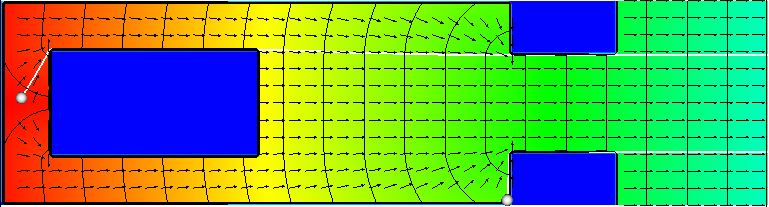
\includegraphics[width=1.\linewidth]{pics/BottleneckObstaclePure}
\caption{Isolines of ``time-cost''.}
\label{fig:BottleneckObstaclePure}
\end{figure}

Given a discretization of the domain \textgreek{W} and the target region ${\partial\Omega}$, the solution to the Eikonal Equation can be approached (angen�hert) by using the Fast-Marching Algorithm. The algorithm provides a first order approximation, yet sufficient for our cause (pedestrian navigation). Computing-time of Fast-Marching is independent\footnote{Fast-Marching completion-time depends mainly on the length of the wavefronts. If the geometry leads to small lengths, as in geometries with large amounts of narrow corridors, completion time decreases.} of the complexity of obstacles and walls. 

The negative gradient $-\nabla u$  of the ``time-cost'' will be a useful tool in the routing of pedestrians/agents to the target region used as part of the algorithm's input. The Fast-Marching algorithm is described in the appendix in detail for further reference.

We will refer to the result of the Fast-Marching Algorithm as ``floor-field''. To successfully use these floor-fields, we will discuss and analyze a modification, which gives us a smooth floor-field, as proposed in roboticslab.uc3m.es.\label{replace with bibtex: http://roboticslab.uc3m.es/roboticslab/researchtopic/fast-marching}

\subsection{Safe Navigation using the Floorfield}

When using the plain approximation to the Eikonal Solution, agents anticipate a non-smooth pathway that leads very close to 
walls (see white trajectories in figure \ref{fig:BottleneckObstaclePure}). In most of the models for pedestrian dynamics, pedestrians, which are very close to walls or obstacles, could overlap with them in rare occasions. Agents might leave the valid domain and find themselves captured inside walls or obstacles. In the model described in this paper, we aim to fix that
problem. In reality, we can observe, pedestrians avoiding walls and obstacles through keeping a certain distance. 

Therefore, it is desirable to define a modified quality of an optimal route, which accounts for a minimal arrival time and a safe pathway. Safe in respect to avoiding the vicinity of walls and obstacles, if and only if possible. If a space is very crowded (high density), then agents should make use of the given space even if that means getting close to walls.

This crowd behavior, described above, is commonly achieved with adding a repulsive characteristic to walls.

In the ``social force model'', the walls will have a repulsive force pointing perpendicular to the wall-surface, aiming to keep agents away from the wall. These forces need to be calibrated to work as intended.

Smaller forces might not be strong enough to avoid overlapping with the wall if an agent is in between a wall on one side and many other agents on the other side. The agents on the other side affect that one agent, forcing him towards the wall, while the wall itself acts on the agent in the opposite direction.

If the repulsive wall forces are too strong, pedestrians will not use the space close to a wall, even if the domain is very crowded.

It is a difficult task, to find a set of parameters, that work as desired in a broad set of situations and geometries.

Instead of modeling the repulsive character of walls (seen as the avoidance of walls by pedestrians) via repulsive wall forces (social force model), we modify the floor-field in a way, that pathways avoid the vicinity of walls to a certain, adjustable degree, thus integrating this repulsive character into the navigation/routing.

How can an agent ``avoid'' the close vicinity of any wall or obstacle?

\subsection{Distances-Field}
\begin{figure}[h!]
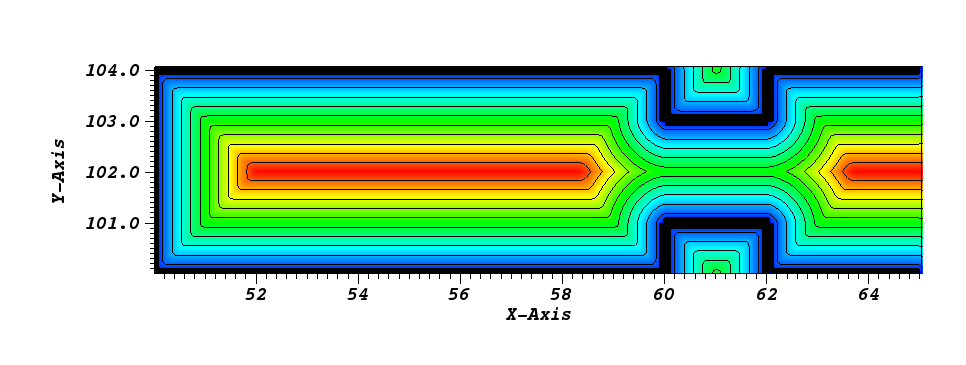
\includegraphics[width=1.\linewidth]{pics/DistanceField2}
\caption{Distances Field of the bottleneck geometry}
\label{fig:DistanceField2}
\end{figure}
Having above question in mind, we first need to introduce and understand the \textit{Distances-Field}, a function $d$ living on the spacial domain $\Omega$, and $d$ holds information, how distant the closest wall is. This function will prove useful when altering the one floor-field, we will use for routing. To avoid confusion, let it be emphasized, that this distances-field will be used in two different parts of the model. It is used to:
\begin{enumerate}
\item create a Direction-to-Wall-Field (vector-field) and
\item to create a slowness-field (scalar-field) to initialize the Fast-Marching algorithm of the Navigation-Field\footnote{ask MC, about denotation of floor-field (vector-field or field of scalars)} (vector-field).
\end{enumerate}

\begin{figure}[h!]
\includegraphics[width=1.\linewidth]{pics/FM_flow}

\caption{Usage of the Distances-Field in the vector-fields}
\end{figure}
\footnote{change "target" to "origin" in figure? easier to understand?}
\paragraph{ad 1:}
The Direction-to-Wall-Field is a normalized vector-field. Each vector has unit length. The orientation is gained by the negative gradient to the Distances-Field. This way, every given vector at $\vec{x}$ directs to the closest wall of that given grid-point $\vec{x}$.
\paragraph{ad 2:}
The function value $d(\vec{x})$ will be used to create a slowness-field on the discrete grid. This slowness-field holds the value, which determines, how slow the 2-D wave will propagate over the grid-point in the final \emph{navigation}-field. Points, that are relatively close to a wall, will have a correspondingly\footnote{outch!} low value $d(\vec{x})$. Therefore, the 2-D wavefront will slow-down over these points. Routes/Pathways passing these points will take more time and be less optimal in a sense, that combines distances and wall-avoidance. We will refer to the value $u(\vec{x})$ as the \emph{time-cost-value} (\emph{cost} in short).


%Both vector-fields, which will have two different names, are created by using the Fast-Marching algorithm:
%\begin{enumerate}
%\item \emph{Direction-to-Wall-Field}: this vector field holds the normalized direction to the closest wall
%\item \emph{Navigation-Field}: this vector field holds the negative gradient of the altered floor-field (time-cost-field)
%\end{enumerate}

%The \emph{Direction-to-Wall-Field} is the normalized Gradient vector-field of the distances. It can be obtained by starting a wavefront $t = 0$ at all grid-points that represent a wall or an obstacle. The wavefront then propagates in the domain with a homogeneous speed. At $ t = 2/v $ the wavefront holds all grid-points, that are $2m$ away from the closest wall.
 
<< explain the pre-step incl. the threshold "cut-off"; have some nice pictures >>

\begin{figure}[h!]
\includegraphics[width=1.\linewidth]{pics/transformFF}
\caption{Isolines of a floor-field (above) compared to isolines of the enhanced floor-field (below). Sample trajectories in white.}
\label{fig:transformFF}
\end{figure}

\subsubsection{Cost of a ``full'' preprocessing step }

Close to all time of the needed computation spent on the enhanced floorfield, the prohibition of overlapping, is spent in a preprocessing step before the actual simulation starts and therefore does not effect the real-time factor. A factor, which is a prominent metric, when comparing different models. In this TEST-model, the preprocessing is increased compared to Dietrich's \emph{Gradient Navigation Model}. Where he uses the Eikonal solution once (mollifiers not considered), the TEST-model uses two runs through the Fast-Marching algorithm. In this chapter we want to elaborate on the doubled effort we spend.

The granularity of the rectangular grid governs the cost of the FM\footnote{Fast-Marching}. For pedestrian navigation, we chose a point-to-point distance of neighboring grid-points of $0.0625 m$. A geometry spanning $100m \times 100m$ can be processed in (enter profiling results). Most of the computing time is spend on the output.

The Fast-Marching algorithm is that fast, that it basically can be neglected when rating the performance. A prequel Fast-Marching run does not change that verdict. The usage of the Direction-to-Wall Field in the model shows no more overlapping and seems easily worth the cost. During runtime, using the floor-field or the Distance-to-Wall field means reading a vector and performing up to 5 scalar products\footnote{to be verified}.

To show the performance of the TEST model, we started a simulation in a complex geometry with more than 3000 agents. Compared to other models available in \emph{JuPedSim}, we could not see any significant performance difference. (ADD PROFILING TIMES, NOT YET EXISTING)
The trajectories improved and look much more natural. This was achieved without the need to manually adding decomposing help-lines or intermediate navigation goals.

\begin{figure}[h!]
\includegraphics[width = 1.\linewidth]{pics/trajCompare}
\caption{Comparison between trajectories: Routing with helplines (left) to routing with navigation field (right).}
\end{figure}

\begin{figure}[h!]
\subfigure{\includegraphics[width=.49\linewidth]{pics/Verteilerebene0}}
\subfigure{\includegraphics[width=.49\linewidth]{pics/Verteilerebene2}}
\subfigure{\includegraphics[width=.49\linewidth]{pics/Verteilerebene4}}
\subfigure{\includegraphics[width=.49\linewidth]{pics/Verteilerebene5}}
\caption{Simulation of a complex geometry with multiple exits and app. 3000 agents}
\label{fig:verteilerebene}
\end{figure}

%\subsubsection{Distances-Field and repulsive Wall-Forces}

%<< optional? describe in short that the distance field takes responsibility for not
%clipping in two ways: redirect in wall-distance < 0.2; modify floor-field to avoid walls >>

%<< move this section >>

%\subsection{Idea of Separation of a Moving-Vector into Direction and Magnitute}

%\subsubsection{no clipping}

%\subsubsection{Recycling the Distances Field (neg. Gradient must be saved)}

%$\vec{v}_{res}\quad=\quad\bigg(1-\frac{1}{2}\bigg[\langle\vec{v}_{n},(-\nabla distances)_{n}\rangle+\big\vert\langle\vec{v}_{n},(-\nabla distances)_{n}\rangle\big\vert\bigg]\bigg)\cdot\vec{v}_{n}$

\section{Validation}
\subsection{Basic Tests}
The validation of a model is a complex task and makes up a separate research field. Researchers in the field of Civil Engineering are working on various approaches on how to validate a model. The research group, CST -  Pedestrian Dynamics and Traffic Simulation, is developing a set of test-cases any serious model should aim to pass. Tests include the behavior of a single moving agent passing static objects like a dummy agent or an obstacle. (see figure \ref{test01})

The TEST-model passed these tests and it was shown, that the basic mechanics of the routing are working as specified.

\begin{figure}[h!]
\includegraphics[width=1.\textwidth]{pics/Testcases01}
\caption{Testcase: Orange agent should pass the (static) blue agent.}
\vspace{1cm}
\includegraphics[width=1.\textwidth]{pics/Testcases02}
\caption{Testcase: Orange agent should pass the (static) blue obstacle.}
\label{test01}
\end{figure} 

%\begin{itemize}
%\item alle oder die wichtigsten Testf�lle
%\item hier auflisten
%\end{itemize}


\subsection{Variation of the Parameter}
In this thesis, we take special interest in the following testcase, as it validates the model to yield a fundamental diagram like seen in real world experiments:
The tests demands to simulate a bottleneck experiment several times. This is to be repeated for various bottleneck-widths. The calculated flow through the bottleneck shall match the empirical data.
We have conducted this test for various \emph{wall-avoid-distance} parameter and want to analyze the change in the flow. It can be seen, that the more the agents will gear to avoid obstacles and walls, the lesser the flow will become. This result is expectable. It was also shown, that without the enhancement of the floor-field, few agents did not pass the bottleneck, but got caught inside of walls.

\begin{figure}[h!]
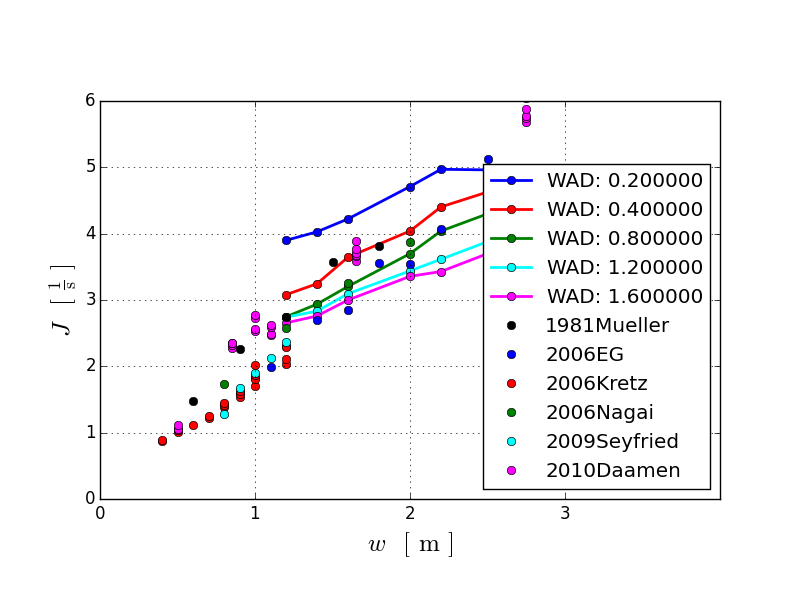
\includegraphics[width=1.\textwidth]{pics/sim_flow_vs_experimental_data}
\caption{Fundamental diagram with empiric data and simulation results}
\end{figure}

\section{Outlook}

In this thesis, an altered usage of an enhanced floor-field was shown, integrated in a suitable new TEST-model. The \emph{wall-avoid-distance} parameter was analyzed and shown to be able to show good convergence to empirical data. During the course of the work process, it became clear how versatile and powerful floor-fields can be. Not only in the current state, they can provide valuable assistance to pedestrian models, but they can be further developed to fit into much more contexts. Any of the outlooks provided in this chapter easily catch my interest and I am already looking forward pursuing the development and seeing how they will improve future simulation suits.

\subsection{Floor-field}

\subsubsection{Multiple Goals }

The floor-field is a useful tool in routing of pedestrians through any geometry. To unfold its full power, one can imagine to calculate a floor-field for each of many goals. The combination of many floor-fields, each corresponding to a goal, can easily be managed by selecting the direction vector of the one floor-field, that provides the minimal time-cost of an active set of floor-fields evaluated at the grid-point of the current agent's position. Dynamic in-world events in a simulation could alter the set of active floor-fields. This way, models can implement navigation in a dynamically changing world. It can be also used, to be a tool in a simulation suit, which has agents change their destination during runtime. This would be realized by simply changing the active set to the floor-fields corresponding to the new destination.

<< Verteilerebene(?) oder etwas kleinere Geometrie mit mehreren Ausg�ngen: Nebeneinander 2-4 Vectorfelder nebeneinander >>

\subsubsection{Multiple Floors}

In the current state, the floor-field provides time-cost on a discrete grid, a rectangular grid with equidistant spacing in each dimension. The grid-points are stored in a one-dimensional array by the row-major order. In a arrangement like this, it is easy to formulate 4-neighboring\footnote{Grid-points north, south, east and west to the current are called 4-neighbors.} relations.  These values are easily accessed, if you are provided the stride value, namely how much grid-points make up the length of both dimensions in a 2-D world. The Fast-Marching algorithm needs the time-cost values of the 4-neighborhood.
This will change, if you need to simulate in a building with multiple floors, which are connected via stairs. We need to introduce a third dimension, which can be treated equally handy inside each floor. Any position, projected onto the x-y-plane, may not be unique anymore. On the other hand, it would be a waste of memory, if a third dimension would be introduced\footnote{As we are interested in points representing the floor of a room, all the volume (air) above would be not used.} introduced, to represent the hull-cube circumscribing a building.
One is to find a solution, which describes the geometry of the rooms in a memory-efficient way and yet be able to comfortably access the 4-neighbors' time-cost value.

%\subsection{Usage in JuPedSim}

%\subsection{Floor-fields in Triangulated Domains}

%\subsection{Parallelization}

\section{Appendices}

\subsection{Fast-Marching Algorithm}


\begin{sequencediagram}
\newthread[white]{u}{User}
\newinst[2]{f}{FloorfieldViaFM}
\newinst[5]{t}{Trial}

  \begin{call}{u}{Create and Init(...)}{f}{}
	\begin{call}{f}{Create and Init(...)}{t}{}
	\end{call}
	\begin{call}{f}{All points are marked unknown}{t}{}
	\end{call}
	\begin{call}{f}{Add target points to narrowband}{t}{}
	\end{call}

    \begin{sdblock}{while narrowband not empty}{}

     \begin{call}{f}{remove minimum from narrowband}{t}{}
     \end{call}
     \begin{callself}{f}{add minimum to know-set}{}{}
     \end{callself}
     \begin{callself}{f}{calc cost of minimum's unknown neighs}{}{}
     \end{callself}
     \begin{call}{f}{add unknown neighbors to narrowband}{t}{}
     \end{call}
   \end{sdblock}
   \begin{callself}{f}{save floorfield}{}{}
   \end{callself}
  \end{call}
\end{sequencediagram}

\subsection{Gradient Model using a Floorfield}

\begin{sequencediagram}
\newthread[white]{u}{User}
\newinst[2]{g}{GradientModel}
\newinst[2]{d}{DirectionStrategy}
\newinst[2]{f}{FloorfieldViaFM}

\begin{call}{u}{Create and Init(...)}{g}{}


\begin{call}{u}{Create and Init(...)}{d}{}
   \begin{call}{d}{Create and Init(...)}{f}{}
   \begin{sdblock}{run simulation}{} 
     \begin{callself}{g}{for each agent}{}{}
       \begin{call}{g}{getTarget()}{d}{return movDir}
         \begin{call}{d}{getDirectionAt()}{f}{return movDir}
         \end{call}
       \end{call}
       
       \begin{call}{g}{getDir2Wall()}{d}{return dir2Wall}
         \begin{call}{d}{getDir2Wall()}{f}{return dir2Wall}
         \end{call}
       \end{call}
       
       \begin{call}{g}{getDistance2Wall()}{d}{return distance2Wall}
         \begin{call}{d}{getDistance2Wall()}{f}{return distance2Wall}
         \end{call}
       \end{call} 
       \begin{callself}{g}{calc moving vector}{}{}
       \end{callself}      
     \end{callself}
   \end{sdblock}
  \end{call}
  \end{call}
\end{call}
\end{sequencediagram}

\subsection{Code Snippets}
\lstinputlisting[label=FFviaFM_h,caption=FloorfieldViaFM Class Header]{../../routing/FloorfieldViaFM.h}
%\lstinputlisting[label=FFviaFM_cpp,caption=FloorfieldViaFM Class Implementation]{../../routing/FloorfieldViaFM.cpp}
\lstinputlisting[label=RectGrid,caption=RectGrid Class Header]{../../routing/mesh/RectGrid.h}
%\lstinputlisting[label=Trial,caption=Trial Class Header]{../../routing/mesh/Trial.h}
%\include{../../math/GradientModel}
\section{Bibliography}
Mohcine's diss

Ulrich's diss

Dietrich's arbeit (introduction)

micro-/macroscopic arbeiten (desktop/READ)

fast-marching arbeiten:
madrid
code

outlook: triangulated version (master/pdfs/fmarcher)

Helbing and Moln�r 1995, Hartmann 2010, Hartmann et al. 2012, ( + Felix 4.2)

history: helbing, ... (einleitungen von mc, uk, fd)

\end{document}
